Un'altra tecnica implementata per il problema di classificazione delle immagini delle TAC al cervello è il \textit{K-Nearest Neighbor}. A differenza della Regressione Logistica, KNN si basa sulla classificazione con decision boundary non lineare.\\
In particolare è importante capire quanti vicini considerare nel modello, ovvero per quale K si ottiene un risultato migliore.
La classe di scikit-learn che permette di implementare l'algoritmo KNN è \textit{KNeighborsClassifier}. Tale classe ha come campo principale il campo \textit{n\_neighbors} che dà possibilità di settare il K dell'algoritmo. Di default il K è pari a 5.
\begin{lstlisting}
from sklearn.neighbors import KNeighborsClassifier

X = brain_tumor_data.drop("Target", axis=1).values
Y = brain_tumor_data["Target"].values
ss = StandardScaler()
X = ss.fit_transform(X)

X_train, X_test, Y_train, Y_test = train_test_split(X, Y, test_size=0.3)

knn = KNeighborsClassifier()
knn.fit(X_train, Y_train)

Y_pred = knn.predict(X_test)
Y_prob = knn.predict_proba(X_test)

acc = accuracy_score(Y_test, Y_pred)
log_loss_score = log_loss(Y_test, Y_prob)

print("ACCURACY: " + str(acc) + "\n")
print("LOG LOSS: " + str(log_loss_score) + "\n")
\end{lstlisting}
Il primo tentativo è quello di effettuare la classificazione KNN con K pari al valore di default, ovvero 5. Si ha un accuracy pari a circa 0.95, mentre il log loss è pari a 0.5 e quindi abbastanza alto.\\
A questo punto si vuole verificare per quale K si ha il risultato migliore in termini di accuracy e log loss. Per fare ciò si implementano più modelli per più K e si visualizzano le metriche su grafici per valutare per quali K il modello ha le migliori prestazioni.\\
L'idea è quella di utilizzare un ciclo for per costruire un modello con K che va da 1 a 20; \textit{Ks} è un array che contiene i diversi valori di K che ad ogni iterazione viene modificato e di seguito si effettuano le fasi di train e di test. A questo punto si calcolano le metriche, ovvero l'accuracy e log loss.
\begin{lstlisting}
Ks = [1, 2, 3, 4, 5, 6, 7, 8, 10, 11, 12, 13, 14, 15, 16, 17, 18, 19, 20]
accuracys = np.array([])
scores = np.array([])
for K in Ks:
print("============ "+"K="+str(K)+" ============")
knn = KNeighborsClassifier(n_neighbors=K)
knn.fit(X_train, Y_train)

Y_pred_train = knn.predict(X_train)
Y_prob_train = knn.predict_proba(X_train)

Y_pred = knn.predict(X_test)
Y_prob = knn.predict_proba(X_test)
Y_pred = knn.predict(X_test)
Y_prob = knn.predict_proba(X_test)

acc = accuracy_score(Y_test, Y_pred)
accuracys = np.append(accuracys,acc)
log_loss_score = log_loss(Y_test, Y_prob)
scores = np.append(scores, log_loss_score)

print("ACCURACY: " + str(acc))
print("LOG LOSS: " + str(log_loss_score) + "\n")
print("===========================================")
\end{lstlisting}
Per il plotting delle metriche in funzione dei diversi K si utilizza semplicemente, ancora una volta, il modulo matplotlib di Python.\\
Nel passo precedente, ovvero nel ciclo for, si salvano le metriche in due array numpy che verranno utilizzati proprio in questo passo.
\begin{lstlisting}
x_plot = np.array(Ks)
y_plot = accuracys
y_plot_2 = scores

plt.plot(x_plot, y_plot, 'r--', label="Accuracy")
plt.xticks(np.arange(x_plot.min(), x_plot.max(), 1))
plt.legend()
plt.show()

plt.plot(x_plot, y_plot_2, 'bs', label='Log loss score')
plt.xticks(np.arange(x_plot.min(), x_plot.max(), 1))
plt.legend()
plt.show()
\end{lstlisting}
\begin{figure}[!htb]
	\minipage{0.45\textwidth}
	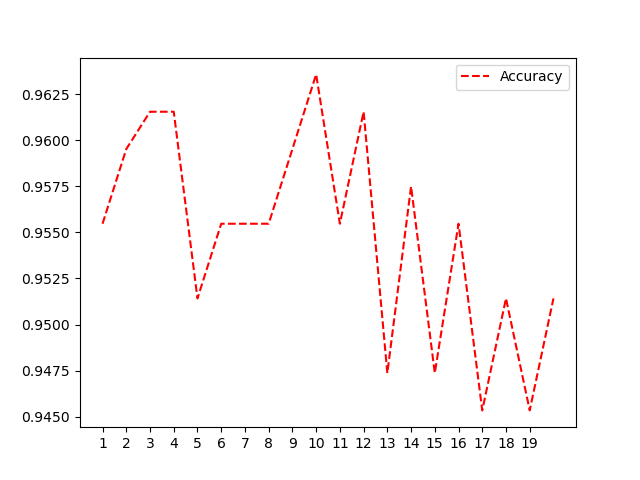
\includegraphics[width=1.2\linewidth]{image/plot_accuracy.png}
	\label{fig:immagine01}
	\endminipage\hfill
	\minipage{0.45\textwidth}
	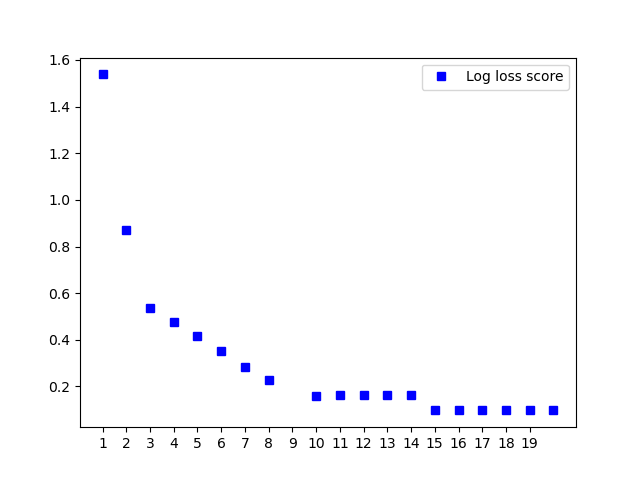
\includegraphics[width=1.2\linewidth]{image/plot_logloss.png}
	\label{fig:immagine2}
	\endminipage
	\caption{A sinistra il plot delle accuracy, a desta quello delle log loss.}
\end{figure}
In termini di accuracy i valori oscillano tra 0.94 a 0.96 con un andamento piuttosto irregolare. In qualsiasi caso, per K che va da 1 a 20 si ha un buon risultato in termini di accuracy.\\
Per quanto riguarda la log loss si nota dal grafico un andamento simile ad un ramo di iperbole. Per K molto bassi (ad es. K = 1 e K = 2) si ha log loss molto alto. All'aumentare del K si ha log loss molto più basso fino a raggiungere un valore limite pari a circa 0.1 per K > 15.
\section{Conclusioni finali sul KNN}
Dal punto di vista dell'accuracy utilizzare un K basso o alto non comporta grosse differenze. Il grafico della log loss suggerisce di utilizzare un K alto in quanto si ha un legame decrescente al crescere di K fino a raggiungere il valore limite.\\
Un buon valore di K per ottenere un ottimo trade off tra accuracy e log loss è 17 (accuracy = 0.96 e logloss = 0.1).